\paragraph{}
In 2008, BIGSSS (Bremen International Graduate School of Social Sciences) was established. Jointly founded by the University of Bremen and Jacobs University, BIGSSS is an interuniversity institution that has obtained initial funding for a period of five years. The Graduate School is part of the Excellence Initiative of the German Federal and State Governments designed to promote science and research. 

\begin{figure}[htbp]
	\begin{center}
		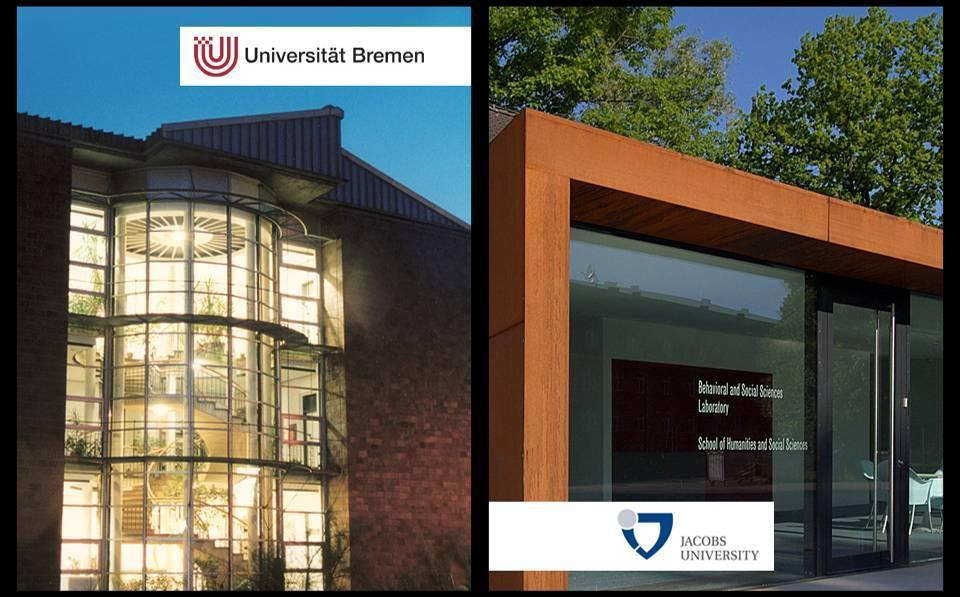
\includegraphics[width=0.5\textwidth,height=5cm]{E:/download/LateX/photo.jpg}
	\end{center}
\end{figure}

Founded upon the core disciplines of political science, sociology and psychology, the School also integrates bordering disciplines. The umbrella theme of BIGSSS is "future social and political integration", encompassing five thematic areas: Global integration; integration and diversity in the New Europe; social integration and the welfare state; attitude formation, value change, and intercultural communication; as well as life course and life dynamics. The JCLL is particularly involved in the field of "Life Course and Life Dynamics", designed to investigate the complex interplay of structure and agency across time, in order to understand changing patterns of societal integration. Currently, two PhD candidates are being trained at the Jacobs Center as part of BIGSSS. Overall, 20 PhD students per year are admitted to BIGSSS, and in addition BIGSSS offers a Post-Doctoral Fellowship Program. At the end of the current 5-year period, BIGSSS will have provided an excellent research basis for over 100 fellows, with more than 50 internationally acknowledged academics facilitating their research activities.  The researchers of BIGSSS are also seeking to establish cooperation with excellent foreign research institutes and universities. 
